\section{Cross-check of the sensitivity with a stand-alone tool}

A separate stand-alone tool that is primarily used to crosscheck and understand SBNfit is also developed. This tool can be used with different test-statistics. When the test-statistic defined in eq.~\ref{eqn:deltachi2} is adopted, the tool is found to perfectly replicate results from SBNFit, providing a useful cross-check of the SBNFit framework. As an additional study, the stand-alone tool is made to employ the ratio of the likelihoods under the two hypotheses as test statistic used to compute the analysis' sensitivity.
Because the statistical test performed involves only a simple hypothesis test, the likelihood-ratio test-statistic can be proven to be the most powerful test, and to outperform the $\Delta\chi^2$.
This test statistic is defined as:
\begin{equation}
\label{eqn:llrpois}
T_{LLR~Pois} = 2 \sum_{i=1}^{N}\left( \mu^i_{H_1} - \mu^i_{H_0} - n^i\log\left(\mu^i_{H_1} / \mu^i_{H}\right) \right)
\end{equation}
where LLR Pois stands for log-likelihood-ratio of the Poisson likelihoods, and the factor of two in front of the expression is just a convention, to make it analogous to the $\chi^2$.
One can see that the $\Delta \chi^2$-like variable is a log-likelihood-ratio, in the Gaussian approximation, and by dropping the term coming from the normalisation factor of the Gaussian formula.
The statistical-only sensitivity measured with the \texttt{LLR Poisson} (eq.~\ref{eqn:llrpois}) test-statistic for the BDT \npsel selection is shown in figure~\ref{fig:1eNp:bdt:sensitivityLLR}. A \textit{p-value} of $0.0019$ is obtained, compared to the value of $0.0032$ with the $\Delta\chi^2$ defined in eq.~\ref{eqn:deltachi2}, demonstrating the larger power of this test-statistic for the simple hypothesis test performed in this analysis.


\begin{figure}[H]
    \centering
    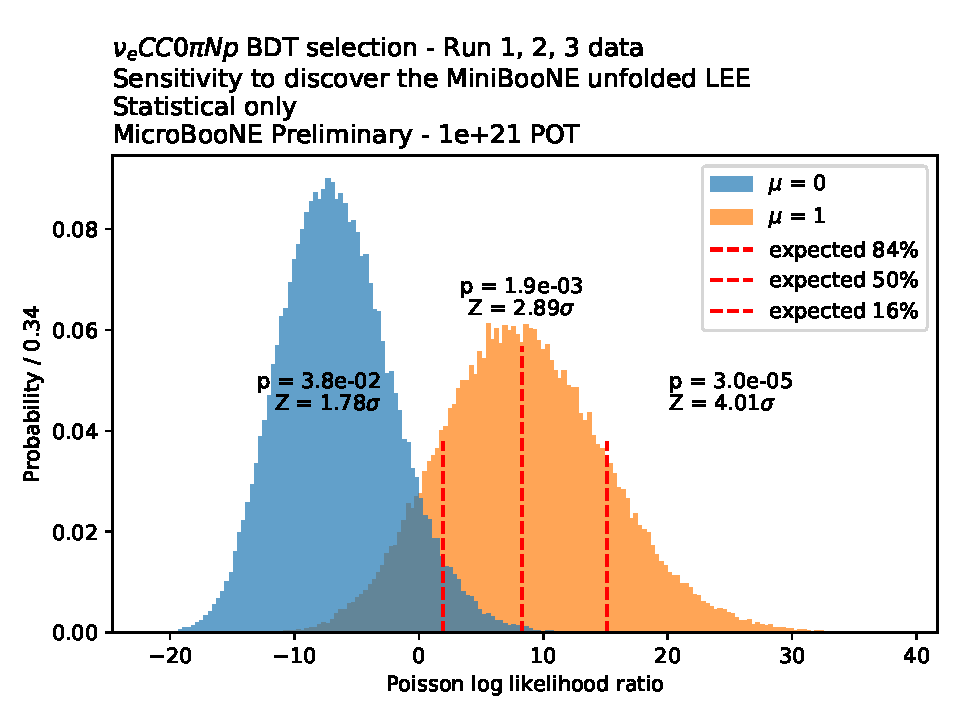
\includegraphics[width=0.5\textwidth]{Sensitivity/pois_llr_test_stat.pdf}
    \caption{Sensitivity calculation for BDT \npsel selection, with the \emph{LLR Pois} test statistic \ref{eqn:llrpois}.}
    \label{fig:1eNp:bdt:sensitivityLLR}
\end{figure}


Using the stand alone tool the expected significance as a function of the collected POT has been computed \ref{fig:sensitivity_function_pot}.
This has been performed using the Poisson LLR test statistic, and including systematic uncertainties as explained previously.

\begin{figure}[H]
    \begin{center}
    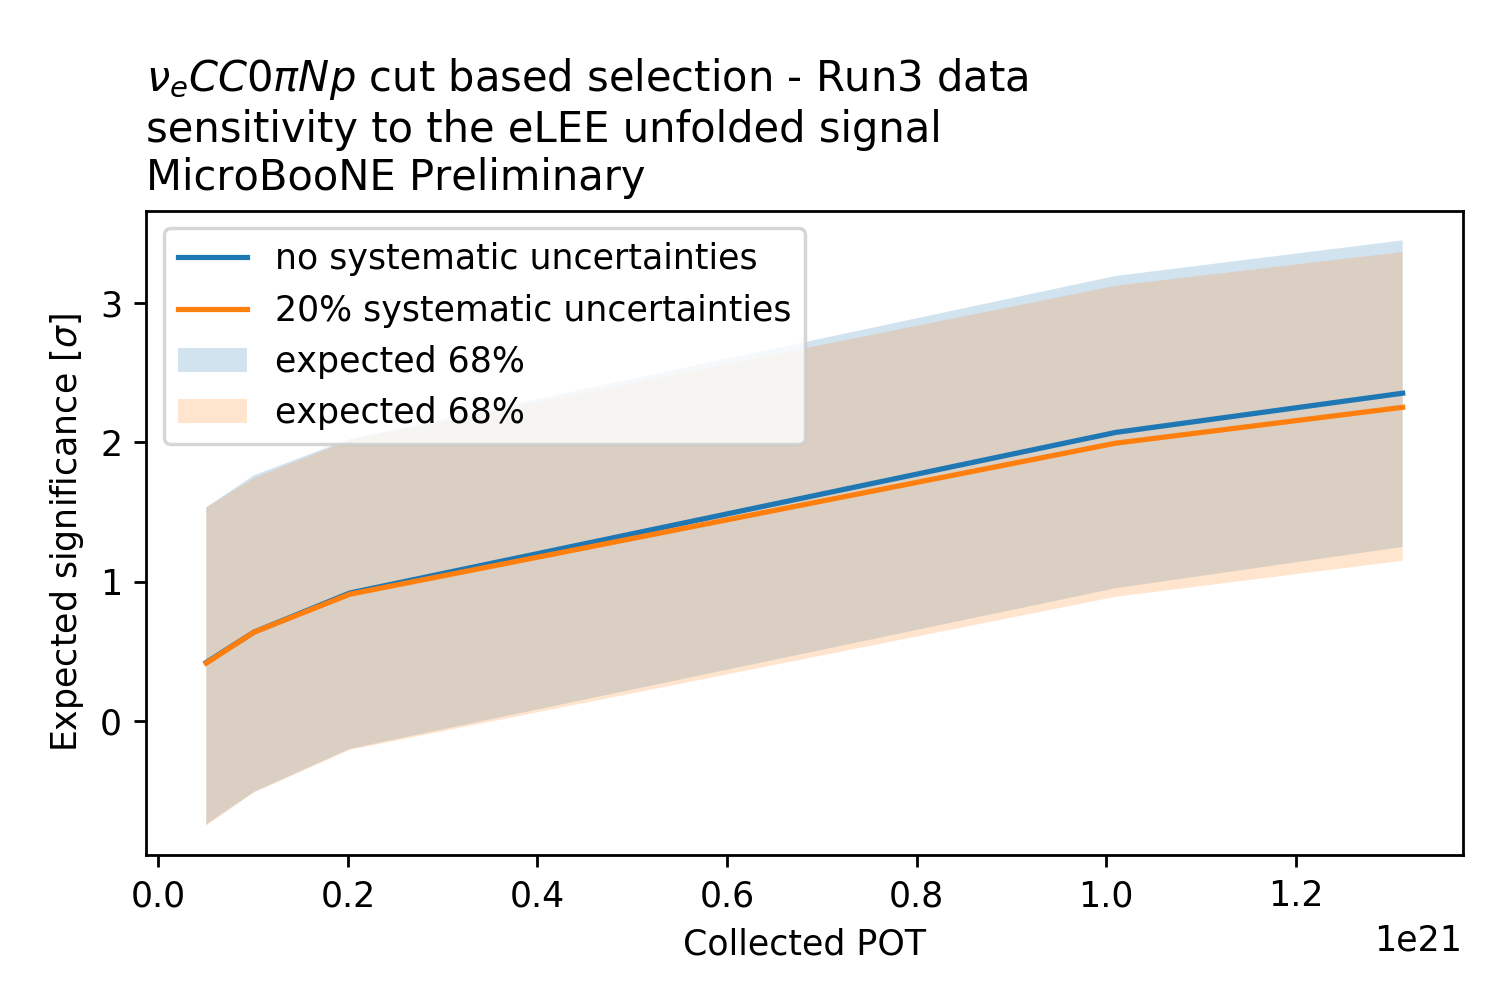
\includegraphics[width=0.5\textwidth]{Sensitivity/sensitivity_vs_pot.png}
    \caption{Expected sensitivity to the LEE unfolded signal, of the \nueccnopinp cut based selection. The solid lines indicate the median values, whereas the shaded regions represent the regions containing 68\% probability.
    The blue (orange) graph shows the case with no (20\%) systematic uncertainty, performed using the stand alone tool as explained previously.
    }
    \label{fig:sensitivity_function_pot}
    \end{center}
\end{figure}

\section{Sensitivity to a 3+1 $\nu_s$ oscillation signal }
In addition to quoting the sensitivity to the MiniBooNE unfolded signal model, the sensitivity to an oscillation signal induced by the presence of a sterile neutrino is studied.
This study is performed within the 3+1 framework, with mass splitting in the $\sim$eV range.
The nature of this analysis, and the strong connection of past short baseline anomalies to sterile neutrino models, makes the investigation of such a hypothesis interesting and relevant for the results' interpretation.
While strong tension exists in global fits to 3+1 signals, this model is less dependent on MiniBooNE's detector and neutrino interaction modeling and therefore provides complementary information enriching the analysis as a whole.
The model under study is a simple extension of the Standard Model with one sterile neutrino.

Despite recognising the interest of this study, we want to acknowledge the main limitations.
So far the oscillation weights are extracted from the flux histograms, assuming a propagation length equal to the distance from the target to the detector.
Taken into account the finite decay length of the parents of the neutrinos would produce an additional smearing in the oscillation probability.
Additionally, the systematic uncertainties are taken into account in an approximate way, by scaling the fractional uncertainties by the oscillation probability.
In fact, the flux uncertainties of the oscillated \nue should be the ones related to the \numu flux, instead of the \nue flux.
All these issues will be taken into account in a further iteration of the study using a dedicated fully oscillated sample.

 
The effective oscillation probability is:
\begin{equation}
\label{eqn:osc_probability}
P^{osc,~short~baseline}_{\mu \rightarrow e} = \sin^2(2\theta_{e\mu})\sin^2\left(1.27 \Delta m^2_{14} \frac{L}{E}\right)
\end{equation}
which  is  characterised  by  an  effective  mixing  parameter  $\sin^2(2\theta_{e\mu})$  and  oscillation  frequency  $\Delta m^2_{14}$.   
The same framework is used to perform a simple hypothesis test and compute sensitivities taking into account the systematic uncertainties on the \nue spectrum after the \numu constraint.  
The assumption is that the \numu disappearance is much smaller than the uncertainties we have on the \numu spectrum, which is true for the values of the oscillation parameters under study.  
No fit or extraction of the oscillation parameters is performed at this stage.  
The parameters value of the best fit to the appearance experiments is chosen, as taken from \cite{bib:oscillation_parameters}.  
The parameters are $\sin^2(2\theta_{e\mu}) = 0.00697$ and $\Delta m^2_{14} = 0.573 \text{eV}^2$.  
The contribution from the oscillation to the expected \nue rate from the BNB is shown in figure \ref{fig:oscillation_event_rate}.


\begin{figure}[ht] 
\centering
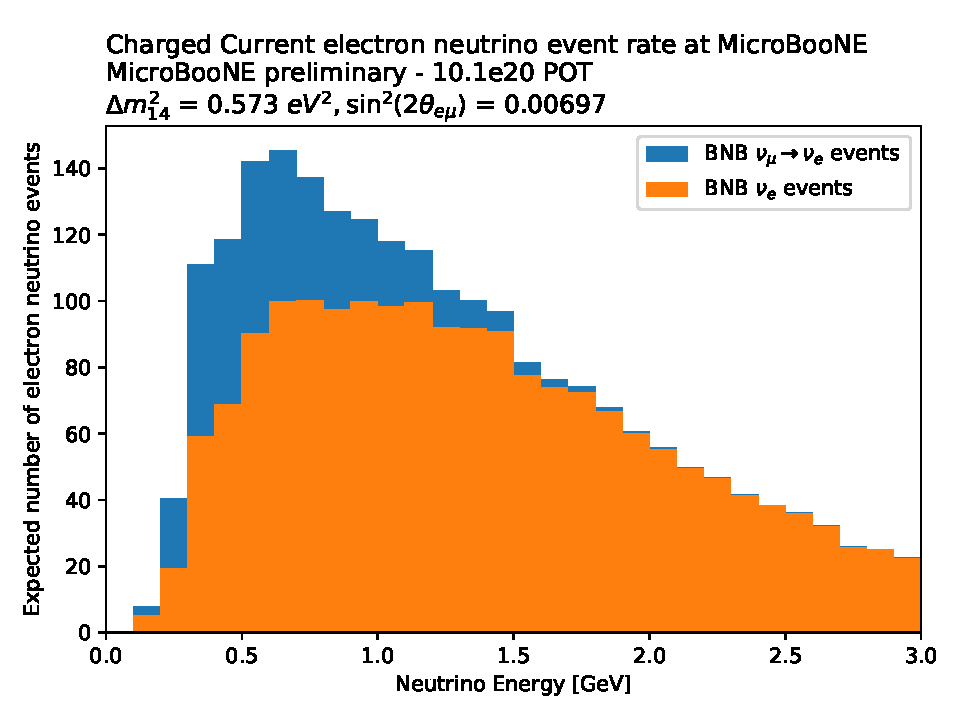
\includegraphics[width=0.45\textwidth]{Sensitivity/oscillation/event_rate_nueccpinp_deltam2_0573_sin2theta2_000697.pdf}
\caption{An additional sterile neutrino at masses much larger than the ordinary neutrinos would induce an effective muon neutrino to electron neutrino oscillation probability. The contribution to the event rate from the \nue intrinsic is shown for the oscillation parameters values $\sin^2(2\theta_{e\mu}) = 0.00697$ and $\Delta m^2_{14} = 0.573 \text{eV}^2$.}
\label{fig:oscillation_event_rate}
\end{figure}



The sensitivity is estimated using the \nueccnopinp BDT selection (sec.~\ref{sec:nueselection:1eNp}). 
The left plot in figure \ref{fig:oscillation_sensitivity} shows the expected reconstructed shower energy spectrum in the presence of the signal. The blue distribution $H_0$ includes both \nue as well as other background events, which can be seen individually in figure \ref{fig:1eNp:bdt:1e21}.
The right plot shows the distribution of the $\Delta \chi^2$ test statistic under the null hypothesis (blue) and oscillation-signal hypothesis (orange), with the expected significance to this signal.

\begin{figure}[H] 
\begin{center}
    \begin{subfigure}[b]{0.45\textwidth}
    \centering
    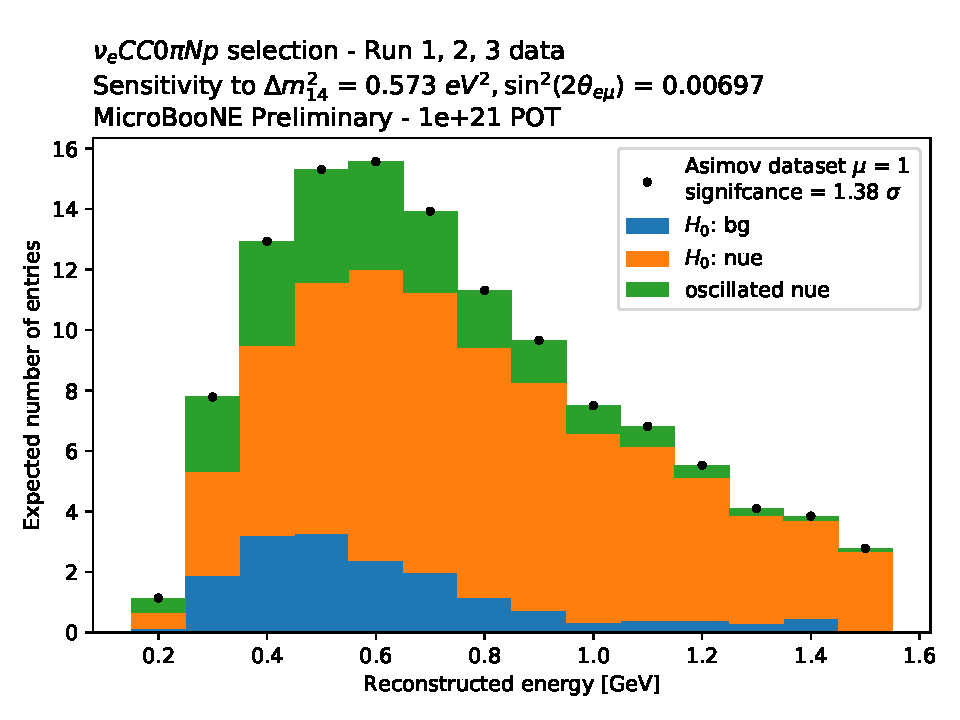
\includegraphics[width=1.00\textwidth]{Sensitivity/oscillation/asimov_nueccpinp_deltam2_0573_sin2theta2_000697.pdf}
    \caption{$E_{reco}$ of the electron candidate shower.}
    \end{subfigure}
    \begin{subfigure}[b]{0.45\textwidth}
    \centering
    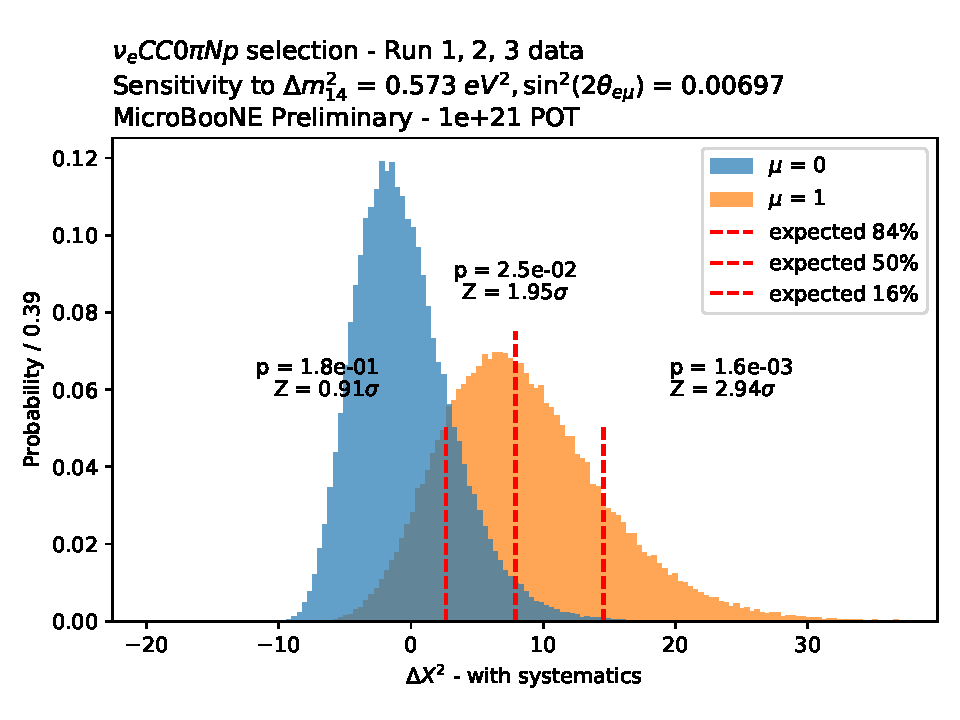
\includegraphics[width=1.00\textwidth]{Sensitivity/oscillation/test_stat_nueccpinp_deltam2_0573_sin2theta2_000697.pdf}
    \caption{$\Delta \chi^2$ test statistic distributions.}
    \end{subfigure}
\caption{Contribution to the spectrum of reconstructed energy energy in the presence of a sterile neutrino (left plot) in the \npsel BDT selection.
The distribution of the test statistic for the null and alternative hypothesis does not show a very large significance for this value of the oscillation parameters. It is important to note however that the selection as designed was not optimized for such a search.}
\label{fig:oscillation_sensitivity}
\end{center}
\end{figure}


While eV sterile neutrinos cause a noticeable effect in the reconstructed \nue spectrum in this analysis, the significance to such models is not strong at the moment. Optimization of the selection cuts can be targeted to enhance sensitivity to an eV sterile neutrino search. This work is a preliminary investigation of the analysis' sensitivity to 3+1 oscillation models and hopefully offers motivation for futher exploration of such models as the analysis progresses.

